\section{Link prediction using Dimensionality Reduction}

The curse of dimensionality is a well-known problem in machine learning.
Some researchers employ dimension reduction techniques to tackle the
above problem and apply it in the \textbf{link prediction} scenario.

\subsection{Embedding-based link prediction}

The network embedding is considered as a dimensionality reduction
technique in which higher \(D\) dimensional nodes (vertices) in the
graphs are mapped to a lower \(d\) (\(d << D\)) \textbf{dimensional
    representation (embedding)} space by preserving the node neighborhood
structures. In other words, \textbf{\emph{find the embedding of nodes to
        a lower d-dimensions such that similar nodes (in the original network)
        have similar embedding (in the representation space)}}.\\ In the Figure
below you can see an application example of a dimensionality reduction
technique to a graph that represent a social network.

\begin{figure}[H]
    \centering
    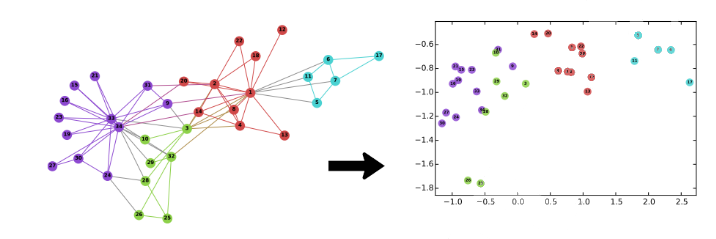
\includegraphics[width=12cm, keepaspectratio]{capitoli/methods/imgs/img4.png}
\end{figure}

The main component of the network embedding is the encoding function or
encoder \(f_{en}\) that map each node to the embedding space
\[f_{en}(x) = z_x\] where \(z_x\) is the \(d\)-dimensional embedding of
the node \(x\). The embedding matrix is \(Z \in R^{d x |V|}\), each
column of which represents an embedding vector of a node.\\

\begin{figure}[H]
    \centering
    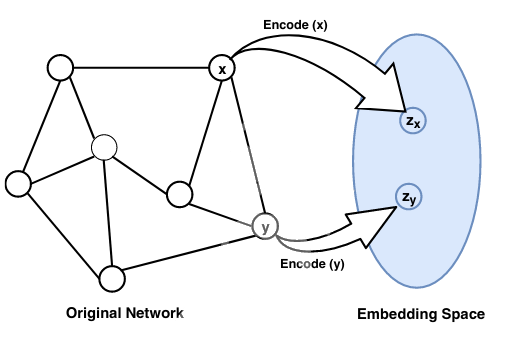
\includegraphics[width=10cm, keepaspectratio]{capitoli/methods/imgs/img5.png}
\end{figure}

Now, a similarity function is \(S(x, y)\) is defined that specifies how
to model the vector (embedding) space relationships equivalent to the
relationships in the original network, i.e.,
\[S(x, y) \approx z_x^T z_y\]

Here \(S(x, y)\) is the function that reconstructs pairwise similarity
values from the generated embedding. The term \(S(x, y)\) is the one
that differ according to the function used in different
factorization-based embedding approaches.\\

For example, \texttt{graph\ factorization} directly employ adjacency
matrix \(A\) i.e.~\((S(x, y) \overset{\Delta}{=} A_{(x,y)})\) to capture
first order proximity, \texttt{GraRep} selects
\((S(x, y) \overset{\Delta}{=} A^2_{(x,y)})\) and \texttt{HOPE} uses
other similarity measures(e.g. Jaccard neighborhood overlap). Most
embedding methods realize the reconstruction objective by minimizing the
loss function, L
\[L = \sum_{(x, y) \in \{V x V \}} l(z_x^T z_y, S(x, y))\]

Once the previous equation is \textbf{converged}
(i.e.~\textbf{trained}), one can use the trained encoder to generate
nodes embedding, which can further be employed to infer missing link and
other downstream machine learning tasks.\\

Recently, some network embedding techniques have been proposed and
applied successfully in link prediction problem. The
\texttt{Laplacian\ eigenmaps},
\texttt{Logically\ linear\ embedding\ (LLE)}, and \texttt{Isomap} are
examples based on the simple notion of embedding. Such embedding
techniques are having quite complex in nature and face scalability
issues. To tackle the scalability issue, graph embedding techniques have
leveraged the sparsity of real-world networks. For example,
\texttt{DeepWalk} extracts local information of truncated random walk
and embeds the nodes in representation space by considering the walk as
a sentence in the language model. It preserves higher order proximity by
maximizing the probability of co-occurrence of random walk of length
\(2k + 1\) (previous and next \(k\) nodes centered at a given node).
\texttt{Node2vec} also uses a random walk to preserves higher order
proximity but it is biased which is a trade-off between the
\texttt{breadth-first\ search\ (BFS)} and
\texttt{depth-first\ search\ (DFS)}.\\

The experimental results show that the \texttt{Node2vec} performs better
than the \texttt{Deepwalk}.\\

In next step, \textbf{Trouillon et al.} introduced complex embedding in
which simple matrix and tensor factorization have been used for link
prediction that uses a vector with complex values. Such composition of
complex embedding includes all possible binary relations especially
symmetric and anti-symmetric relations. Recently, some more studies have
been published in link prediction using embedding, for example,
\textbf{Cao et al.~subgraph embedding}, \textbf{Li et al.~deep dynamic
    network embedding}, \textbf{Kazemi et al.}, etc.

\subsection{Matrix factorization/decomposition-based link prediction}

From last decade, matrix factorization has been used in lots of papers
based on link prediction and recommendation systems. Typically, the
latent features are extracted and using these features, each vertex is
represented in latent space, and such representations are used in a
supervised or unsupervised framework for link prediction. To further
\textbf{improve the prediction results, some additional node/link or
    other attribute information can be used}. In most of the works,
non-negative matrix factorization has been used. Some authors also
applied the singular value decomposition technique. Let the input data
matrix is represented by \(X = (x_1, x_2, ..., x_n)\) that contains
\(n\) data vectors as columns. Now, factorization of this matrix can be
expressed as \[X \approx FG^T\] where
\(X \in R^{p x n}, F \in R^{p x k} , and G \in R^{n x k}\) . Here, \(F\)
contains the bases of the latent space and is called the basis matrix.
\(G\) contains combination of coefficients of the bases for
reconstructing the matrix \(X\) , and is called the coefficient matrix.
\(k\) is the dimension of latent space \((k < n)\). Several well-known
matrix factorizations are expressed based on some constraints on either
of the three matrices, for example

\begin{itemize}
    \item \texttt{SVD}:
          \(X_\pm \approx F_\pm G_\pm^T\)
    \item \texttt{NMF}:
          \(X_+ \approx F_+ G_+^T\)
    \item \texttt{Semi-NMF}:
          $X_\pm \approx F_\pm G_+\^{T} $
    \item \texttt{Convex-NMF}:
          $X_\pm \approx  X_\pm W_+ G_\pm^{T}$
\end{itemize}

In the above four equations, \(Z_\pm\) represents the nature of the
entries in the matrix \(Z\), i.e.~both positive and negative entries
allowed in the matrix \(Z\). In the last equation, \(F = XW\) represents
the convex combinations of the columns of \(F\) . Generally, such a
factorization problem can be modeled as the following
\texttt{Frobenius\ norm\ optimization\ problem}
\[min_{f, g} ||X - FG^T||^2_{fro}\]
\[\text{subject to} F \ge 0, G \ge 0\] Here \(||Z||^2_{fro}\) is the
frobenius norm of \(Z\) and the constraints represent NMF factorization.
However, any of the above four constraints can be used depending on the
requirement of the problem underlying. After solving the above
optimization problem, the similarity between a non-existing pair
\((x, y)\) can be computed by the similarity of the \(x^{th}\) and
\(y^{th}\) row vectors in the coefficient matrix \(G\).

\begin{itemize}
    % \tightlist
    \item
          \texttt{Acar\ et\ al.} expressed temporal link prediction as a matrix
          completion problem and solve it through the
          \texttt{matrix\ and\ tensor\ factorization}. They proposed a weighted
          method to collapsed the temporal data in a single matrix and factorize
          it using \texttt{CANDECOMP/PARAFAC\ (CP)} tensor decomposition method.
    \item
          \texttt{Ma\ et\ al.} also applied matrix factorization to temporal
          networks where features of each network are extracted using
          \texttt{graph\ communicability} and then collapsed into a single
          feature matrix using \texttt{weighted\ collapsing\ tensor\ (WCT)}.
          They showed the equivalence between eigen decomposition of
          \texttt{Katz\ matrix} and
          \texttt{non-negative\ matrix\ factorization\ (NMF)} of the
          communicability matrix that serves as the foundation of their
          framework.
    \item
          \texttt{Menon\ et\ al.} proposed a work for structural link
          prediction. Here, the problem is modeled as
          \texttt{matrix\ completion\ problem}, and
          \texttt{matrix\ factorization} are used to solve it. They introduced a
          supervised matrix decomposition framework that learns latent
          (unobserved) structural features of the graph and incorporates it with
          additional node/link explicit feature information to make a better
          prediction. Additionally, they allowed the factorization model to
          solve class imbalance problem by optimizing ranking loss.
    \item
          \texttt{Chen\ et\ al.} proposed a work, where the authors extracted
          topological matrix and attribute matrix and factorized these matrices
          using \texttt{non-negative\ matrix\ factorization}. The final score
          matrix is obtained by integrating these two matrices in the latent
          space.
\end{itemize}